\documentclass{article}

\usepackage{amsmath, amsthm, amssymb, amsfonts}
\usepackage{thmtools}
\usepackage{graphicx}
\usepackage{setspace}
\usepackage{geometry}
\usepackage{float}
\usepackage{hyperref}
\usepackage[utf8]{inputenc}
\usepackage[english]{babel}
\usepackage{framed}
\usepackage[dvipsnames]{xcolor}
\usepackage{tcolorbox}
\usepackage{enumitem}
\usepackage{tikz}
\usepackage{tikz-3dplot}
\usepackage{graphicx}
\usepackage{biblatex}

\addbibresource{bibliography.bib}

% \colorlet{LightGray}{White!90!Periwinkle}
\colorlet{LightGray}{Blue!30}
\colorlet{LightOrange}{Orange!15}
\colorlet{LightGreen}{Green!15}

\newcommand{\HRule}[1]{\rule{\linewidth}{#1}}

\declaretheoremstyle[name=Theorem,]{thmsty}
\declaretheorem[style=thmsty,numberwithin=section]{theorem}
\tcolorboxenvironment{theorem}{colback=LightGray}

\declaretheoremstyle[name=Proposition,]{prosty}
\declaretheorem[style=prosty,numberlike=theorem]{proposition}
\tcolorboxenvironment{proposition}{colback=LightOrange}

\declaretheoremstyle[name=Principle,]{prcpsty}
\declaretheorem[style=prcpsty,numberlike=theorem]{principle}
\tcolorboxenvironment{principle}{colback=LightGreen}


\makeatletter
\renewcommand{\maketitle}{%
  \begin{center}
    \vspace*{3cm} % Adjust the vertical space as needed
    {\LARGE\@author\par}
    \vspace{1cm} % Adjust the vertical space as needed
    {\Huge\bfseries\@title\par}
    \vspace{2cm} % Adjust the vertical space as needed
    {\Large\@date\par}
  \end{center}
}
\makeatother


\begin{document}

\title{ \normalsize \textsc{}
\\ [0.5cm]
\HRule{1.0pt} \\
\Huge \textbf{The Evasion Problem}
\HRule{1.0pt}
\\ [1.5cm]
\LARGE{Andrej Jočić \\ Matija Ojo}
}
\author{\textbf{Computational Topology - group project}}
\date{\today}

\maketitle

\newpage


\section{Introduction}

The evasion problem asks if there is a way to move in an area covered with moving sensors while avoiding detection.
We assume the sensors follow predefined paths and their movement is periodic.
This means that the positions and movement directions of the sensors (and thus the area they cover) repeats itself after some global period, which is often the case with real sensor configurations.
Furthermore, we assume the area in question is a subspace of the plane $ \mathbb{R}^2 $, however this is not necessary, since the method presented here can be trivially generalized to higher dimensions as well.

Aside from validating sensor configurations, this can be used to determine the minimal number of sensors (and their movement paths) needed to guarantee detection of an intruder.
Clearly this could be achieved by covering the entire area with sensors at all times, but we can cut costs if we only want to make sure the intruder is detected {\it at some point} during the sensor movement cycle.

To ease implementation at the cost of some generality, we make the following simplifying assumptions:
\begin{itemize}
  \item the intruder's movement speed is unbounded,
  \item the area in question is a rectangular grid,
  \item the paths along which the sensors move are straight line segments,
  \item all sensors move at the same speed of one unit of distance per one unit of time, and
  \item each sensor covers a square area two units of distance across oriented parallel to the edges of the room they protect.
\end{itemize}


\section{Methods}

By considering the unobserved (free) area at each point in time $t \in \mathbb{R}$ (a two-dimensional planar slice), we obtain the three-dimensional {\it free complex} $F$ embedded in space-time.
We are only interested in the times up to the (global) sensor network period $p$, since the object simply repeats itself after $p$.
Therefore, the complex we obtain is similar to a torus, where the first point in time is ``glued'' to the time at $t = p$.
One way to obtain the evasion paths would be to compute $ H_1 (F, \mathbb{Z}) $ and check which generators represent valid cycles/paths (i.e. cycles going strictly forward in time).
However, we decided to take a different approach: collapsing the free complex to a directed graph and computing cycles from its starting nodes. Before discussing that, we will first describe the data structures used to represent the input and the free complex (the code can be found in the project repository \cite{githubrepo}).

\subsection{Sensors}

Since all the sensors have the same properties (area covered, speed of movement), they are uniquely defined by the \texttt{Path} which they follow.
A \texttt{Path} is a sequence of \texttt{Position}s, where a \texttt{Position} is point in the plane $(x, y)$.
Since we want the sensors to move along straight line segments, two consecutive \texttt{Position}s need to either have equal $x$ or equal $y$ coordinates.
The length of a \texttt{Path} is the sum of all the consecutive line segments that form it.
Sensors move towards the next defined \texttt{Position} in the \texttt{Path}, and move towards the first \texttt{Position} when reaching the last one.

The \texttt{SensorNetwork} class is a collection of \texttt{Sensor}s along with the width and height of the rectangular area.
\texttt{SensorNetwork} represents the entire configuration of the input, since the behaviour of the system is determined by the initial situation.
The global period of the system ($p$) is computed as the least common multiple of all the sensor \texttt{Path}'s lengths.

\subsection{Free complex} \label{sec:free_complex}

Due to the space discretization and axis-aligned sensor paths, the most suitable data structure for the free complex $F$ is a cubical complex.
We used the \href{https://gudhi.inria.fr/python/latest/cubical_complex_user.html}{\texttt{CubicalComplex}} from the \href{https://pypi.org/project/gudhi/}{gudhi} library, which only allows axis-aligned cuboids.

We can simplify the complex construction by not taking any {\it wedge shapes} into account.
A wedge shape is a situation where a cell in the grid was covered at time $t$, but is not covered at time $t + 1$ or vice versa - not covered at $t$, but covered at $t + 1$.
This would result in cuboids that aren't axis-aligned, as seen in Figure \ref{fig:wedge}.
We can omit those shapes, because the intruder trying to avoid detection can either be in a particular cell or not - we do not allow partial occupation of a cell.
Therefore, the valid positions for the intruder in the time interval $[t, t + 1)$
are only those which are not covered at the two consecutive times $t$ and $t + 1$.

\smallskip

\begin{figure}[H]
  \centering

  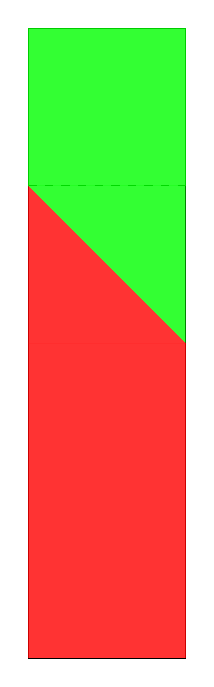
\begin{tikzpicture}[scale=2,transform shape]
    \draw (0,0) rectangle (1,4);
    \draw[dashed] (0,3) -- (1, 3);

    \fill[red, opacity=0.8] (0,0) rectangle (1, 2.001);
    \fill[red, opacity=0.8] (0, 2) -- (1, 2) -- (0, 3) -- cycle;
    \fill[green, opacity=0.8] (1,2) -- (1,3) -- (0,3) -- cycle;
    \fill[green, opacity=0.8] (0, 3) rectangle (1, 4);
  \end{tikzpicture}

  \caption{Top-down representation of a wedge shape in a cubical complex, with time increasing to the right. The covered area is shown in red and the free area is shown in green. In this case a cell was covered at time $t$ but no longer covered at time $t + 1$.}
  \label{fig:wedge}
\end{figure}

The covered planar slices are obtained by performing a union on all the covered areas by all sensors at each point in time.
Covered area is simply a \texttt{Position} representing the top-left corner of a covered cell.

The cubical complex of dimensions $ room\_width \times room\_height \times period $ is constructed by assigning the filtration value of $1$ to free top-dimensional cells and $0$ to covered cells.
According to the reasoning described above, a cell in the complex is marked free {\it iff} the corresponding space is free at two consecutive time-steps $t$ and $t + 1$ (corresponding to 2 faces of the cube in $F$).

\begin{figure}[H]
  \centering
  \includegraphics[width=0.7\linewidth]{example_cubical_complex.png}
  \caption{Free cubical complex of the example configuration (shown in Figure \ref{fig:example}).}
  \label{fig:example_cub_complex}
\end{figure}


\subsection{Computing evasion paths}

Once the cubical complex $F$ is obtained,
we collapse it into a graph (1-dimensional complex) $G$ in a way that preserves $H_1(F)$.
A proper elementary collapse would have to preserve higher-dimensional homology as well, however we are only interested in $H_1(F)$.
Incidentally, $F$ shouldn't have any $H_2$ generators (enclosed caves) in the case of continuous sensor movement; this would imply there is something homeomorphic to a ball in the covered complex, meaning at some time $t_0$ one or more sensors appear out of thin air, and then disappear into a point at time $t_1 > t_0$.
% TODO: proof that H_1 (and H_0) is preserved?

The vertices of $G$ correspond to connected components (by 4-connectivity) of $F$ at each time interval $[t, t + 1)$, $0 \leq t < p$.
The idea is that an intruder with unbounded speed can move between any pair of points in a connected component of free space within a finite time interval without being detected.
The vertices are labeled with $(t, c)$ where $c$ is the index of the connected component in this time slice,
and they also hold information about the area they cover (so that we can obtain concrete \texttt{Position}s after computing a cycle).

Edges in $G$ allow the intruder to move forward in time, so an edge from $(t, c)$ to $(t + 1, c')$ is added {\it iff} the connected areas $c$ and $c'$ intersect (and thus the intruder can move from $c$ to $c'$ in one time step).
If we wanted to strictly follow the homology approach to this problem, these edges would need to be undirected so that we end up with a simplicial complex on which to compute $H_1$.
But in order to avoid having to filter out cycles that don't go forward in time, we kept track of the direction of edges in $G$.

\begin{figure}[H]
  \centering
  \includegraphics[width=\textwidth]{example_graph.png}
  \caption{Evasion graph $G$ of example sensor configuration (shown in Figure \ref{fig:example}). Vertices are horizontally sorted by time. Note there are a few edges going seemingly backwards in time, but they are actually going forward in time, since the time is modulo the period.}
  \label{fig:example_graph}
\end{figure}

Cycles of $G$ are then obtained by performing a depth-first search (with depth limited to $p$) on the graph and checking whether the current node is equal to the starting node.
The above construction guarantees that each cycle in $G$ corresponds to a valid evasion path of length $p$.

Note that this method can be easily generalized to higher dimensions, since a higher-dimensional cubical complex can be collapsed to a graph in the same manner. For example, evasion paths in 3-dimensional space can be computed by dividing the 3-dimensional slices of a 4-dimensional complex into connected components, and connecting the vertices along the 4th dimension.
Beyond that, we could perhaps model configuration spaces with even more dimensions.

\section{Results}

We tested the algorithm with several configurations.
The first configuration is trivial: a single sensor moving in the counter-clockwise direction (Figure \ref{fig:ccw}).
\begin{figure}[H]
  \centering
  \includegraphics[width=0.3\linewidth]{ccw.png}
  \caption{Counter-clockwise circular sensor in 4x4 room, period: 8}
  \label{fig:ccw}
\end{figure}

The algorithm correctly found 1 evasion path, an animation of which can be found \href{https://github.com/MOj0/TDA_Evasion/blob/main/report/ccw.gif}{here}.
% \bigskip
The next configuration is the example from the instructions (Figure \ref{fig:example}).
\begin{figure}[H]
  \centering
  \includegraphics[width=0.6\linewidth]{example.png}
  \caption{6 sensors in 8x8 room, period: 40}
  \label{fig:example}
\end{figure}

The algorithm found 288 different evasion paths through components of free space; an animation of one such path can be found \href{https://github.com/MOj0/TDA_Evasion/blob/main/report/example.gif}{here}.

\bigskip

Lastly, we tested the algorithm on random inputs, such that every point in the room is covered by at least one sensor at least part of the time.
Here are some inputs, along with their animations:

\begin{itemize}
  \item $10 \times 13$ room with 30 sensors, and a period of 80, where the algorithm found a single evasion path; an animation of the path can be found \href{https://github.com/MOj0/TDA_Evasion/blob/main/report/random_sensor_network_10x13_s30_p80_e1.gif}{here}.
  \item $12 \times 18$ room with 48 sensors, and a period of 56, where the algorithm found 2 evasion paths; an animation of one path can be found \href{https://github.com/MOj0/TDA_Evasion/blob/main/report/random_sensor_network_12x18_s48_p56_e2.gif}{here}.
  \item $12 \times 24$ room with 58 sensors, and a period of 84, where the algorithm found 68 evasion paths; an animation of one path can be found \href{https://github.com/MOj0/TDA_Evasion/blob/main/report/random_sensor_network_12x24_s58_p84_e68.gif}{here}.
  \item $20 \times 18$ room with 66 sensors, and a period of 80, where the algorithm found 247125 evasion paths; an animation of one path can be found \href{https://github.com/MOj0/TDA_Evasion/blob/main/report/random_sensor_network_20x18_s66_p80_e247125.gif}{here}.
\end{itemize}


\section{Discussion}

We implemented evasion path detection by using the cubical complex structure, reducing it to a graph and finding the cycles there.
This is equivalent to computing the $ H_1(F, \mathbb{Z})$ on the free complex, however this way we did not need to handle edge cases relating to time travel.

We also implemented sensor paths formed of arbitrary line segments, and a room generator that creates areas of random sizes and sensor configurations.
Lastly, we implemented animations of evasion paths which help to visually confirm the algorithm's correctness.

There is, however, a limitation to the algorithm that we only briefly discussed in Section \ref{sec:free_complex}.
Since we only allow axis-aligned cuboids in the \texttt{CubicalComplex} (i.e. no diagonal edges), the algorithm is not able to detect \textit{tight} evasions.
By tight evasion we refer to the intruder's movement in free space that is covered by sensors in the previous and/or next integer time step. An intruder modeled as a single point in space {\it can} perform such an evasion, so we can just say we are modelling the intruder as a unit square that is dragging a cape behind it (which can still be briefly detected after the intruder has moved on).

This was done due to a limitation of the \texttt{CubicalComplex} in the gudhi library, so detection of tight evasions would require a different data structure for the free complex.
Furthermore, the algorithm for collapsing the complex to a graph should be changed, such that the nodes of the graph are in time slices instead of time intervals, and the edges span through intervals.

\subsection*{Alternative approaches}

Instead of collapsing the cubical complex to a graph, we could have computed $H_1$ generators of the free complex directly and then checked which ones correspond to valid evasion paths. To our knowledge, there is no software that can compute $H_1$ generators of a cubical complex, so we
would first have to subdivide the cubical complex into a simplicial one (dividing squares into triangles and cubes into tetrahedra). Of course, we could also have implemented cubical homology computation ourselves, but that would require a lot of time and effort for something that would almost certainly take longer to compute evasion paths than the approach we took.

An alternative homology-based approach would be to
represent the time-varying (2-dimensional) free space with a zig-zag filtration and derive evasion paths from zig-zag persistence information \cite{Adams_2014}.


\section{Bibliography}

\printbibliography

\end{document}